\section{透過光スペクトルのモデリング}

\begin{figure*}[htb]
\begin{center}
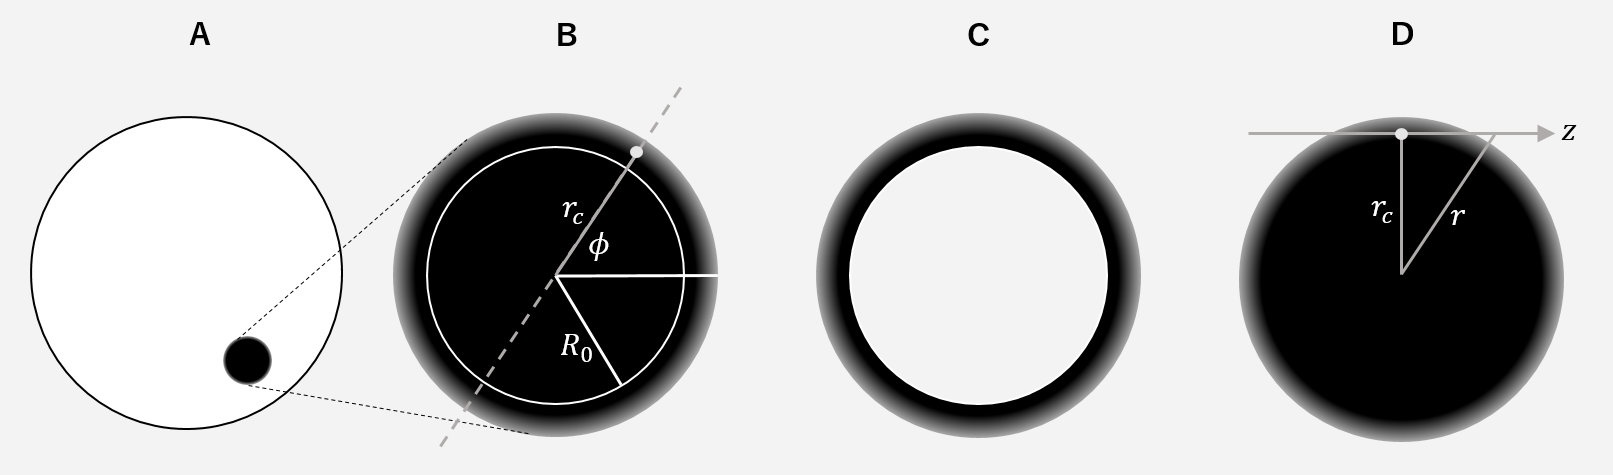
\includegraphics[width=0.85\linewidth]{fig/transmission_chord.PNG}
\caption{透過光分光を考えるための座標系。A:恒星の前面を通過する惑星。B:惑星部分の拡大図。C:円環影部分。D:中の破線方向に惑星を切断したときの図。恒星光の通過方向である$z$方向を弦方向と呼んでいる。右図は「系外惑星探査」図4.13に対応している。\label{fig:transmission_chord}}
\end{center}
\end{figure*}

図\ref{fig:transmission_chord}がトランジット時の概念図である。
透過光で問題になるのは惑星半径付近の薄い大気層での透過率の波長依存性である。そこで、十分透過率が低い位置の基準半径$R_0$を定めてそこから上層までの大気層の円環成分(図\ref{fig:transmission_chord}C)の実効的な影面積$A(\lambda)$(以降、円環影と呼ぶ)を考える。


例えばトランジット深さだけ考える場合、波長$\lambda$での惑星半径と恒星半径を$R_p(\lambda)$,$R_\star(\lambda)$であるとして
\begin{align}
\delta(\lambda) = \frac{R_p^2(\lambda)}{R_\star^2(\lambda)}  = \frac{\pi R_0^2 + A(\lambda) }{\pi R_\star^2(\lambda)}    
\end{align}
が観測量となり、円環影部分のみを考えればよい\footnote{Ingress/Egressを考える場合は円環影の一部分しか透過光に寄与しないためより複雑となるがここでは考えない。}。



さて一般に円環影部分(図\ref{fig:transmission_chord}C)の計算を考えよう。
座標系を図\ref{fig:transmission_chord} B/Dのように取る。
円環影部分は
\begin{align}
A &= \int_0^{2 \pi} \int_{R_0}^\infty [ 1 - \mathcal{T}_\lambda(r_c, \phi)] r_c d r_c d\phi \nonumber \\
&= \pi \left( 2 \int_{R_0}^\infty [ 1 - \mathcal{T}_\lambda(r_c, \phi)] r_c d r_c  \right)
\end{align}
また、
\begin{align}
    \label{eq:rp_trans}
    R_p(\lambda) = \sqrt{ R_0^2 + 2 \int_{R_0}^\infty [ 1 - \mathcal{T}_\lambda(r_c, \phi)] r_c d r_c }
\end{align}
とあらわされる。ここに$\mathcal{T}_\lambda(r_c, \phi)$は、ある波長$\lambda$における惑星ディスク半径$r_c$での弦方向の透過率である。$\mathcal{T}_\lambda(r)$は弦方向の光学的厚さ$t$と
\begin{align}
  \mathcal{T}_\lambda(r_c) = e^{-t}
\end{align}
の関係にある。以降、表記の簡略化のため$\lambda$の添え字を省略する。

$t$は弦方向の座標を$z$と取り、
\begin{align}
    t(r_c) = \int_{-\infty}^\infty \kappa(r) \rho(r) dz = 2 \int_{0}^\infty \kappa(r) \rho(r) dz
\end{align}
である。さてこの積分を大気レイヤーモデルで評価していこう。$t_n$を$n$番目のレイヤーの弦方向のオパシティとする。
図\ref{fig:transmission_coord}より
\begin{align}
    t_n &= 2 \sum_k \kappa_k \rho_k \Delta z^{(n)}_k 
\end{align}
この$\Delta t^{(n)}_k$は$n$番目のレイヤにむかってはられた弦方向の$k$ - $k-1$間レイヤーのオパシティである。これを鉛直一次元方向のオパシティ$\Delta \tau_k = \kappa_k \rho_k \Delta r_k$と関係づけると
\begin{align}
    t_n &= \sum_k  C_{nk} \Delta \tau_k \\
    \label{eq:chord_geo_matrix}
    C_{nk} &\equiv \frac{2 \Delta z^{(n)}_k}{\Delta r_k}
    = 2 \frac{\sqrt{r_{k-1}^2 - r_{n}^2} - \sqrt{r_{k}^2 - r_{n}^2}}{r_{k-1} - r_{k}}
\end{align}
となる。また$r_{N-1}=R_0$である。ここに下三角行列であるChord Geometric matrix $C = \{ C_{nk} \}$を要素ごとに定義した。

$N$は総レイヤー数($n=0,1,\cdots,N-1$)とする。
各レイヤー(下側境界までの)半径とレイヤーの高さには
\begin{align}
r_{n-1} = r_n + \Delta h_n
\end{align}
の関係がある。境界条件は、大気レイヤーの最下層を$n=N-1$とし、$R_0 = r_{N-1}$を惑星中心から最下層の下側境界までの基準半径とする。$r_{N-1}$より下は光が全く透過しないとする。すなわち
\begin{align}
    r_{n} =
\left\{
\begin{array}{ll}
\sum_{j=N-1}^{n+1} h_j + R_0 & \mbox{\, for $j<N-1$} \\
R_0 & \mbox{\, for $j=N-1$} 
\end{array}
\right.
\end{align}
となる。また$n=0$のレイヤーの上側境界(Top of Atmosphere; TOA)が必要である。これは別途$r_\mathrm{top}$と表記する。

大気レイヤーは$(T_n,P_n)$で表記されているため、長さスケールをスケールハイトを用いて変換しないとならない
\begin{align}
\Delta h_n &=  H_n \frac{\Delta P_n}{P_n} \\
\label{eq:H_each}
 H_n &= \frac{k_B T_n}{g_n \mu_n m_H} 
\end{align}
また重力定数は
\begin{align}
g_n = \frac{G (M_p + \Delta M_n)}{r_n^2}
\end{align}
と表される。$\Delta M_n = \sum_{j=N-1}^n \Delta m_j$であり$m_j$は$j$番目のレイヤの持つ質量である。$\Delta M_n$自体は通常は$M_p$に比べて無視できるので考えなくても良いかもしれない。

数値的には最下層から順番に$n=N-1, N-2, \cdots, 0$について$\Delta h_n, r_n$を解いていけばよい。境界条件は$r_N = R_0, g_N = G M_p/r_N^2$である。また$h_0 = 0$として最上層のオパシティは含めない。また同時に各層ごとに$C_{nk}$を$k=n$から$k=N-1$まで計算をしておけば、Chord Geometric Matrix が計算できる\footnote{もちろん$r_n$を計算した後に式(\ref{eq:chord_geo_matrix})で一括で計算してもよい。}。このように$C$は三角行列である。

\begin{figure*}[htb]
\begin{center}
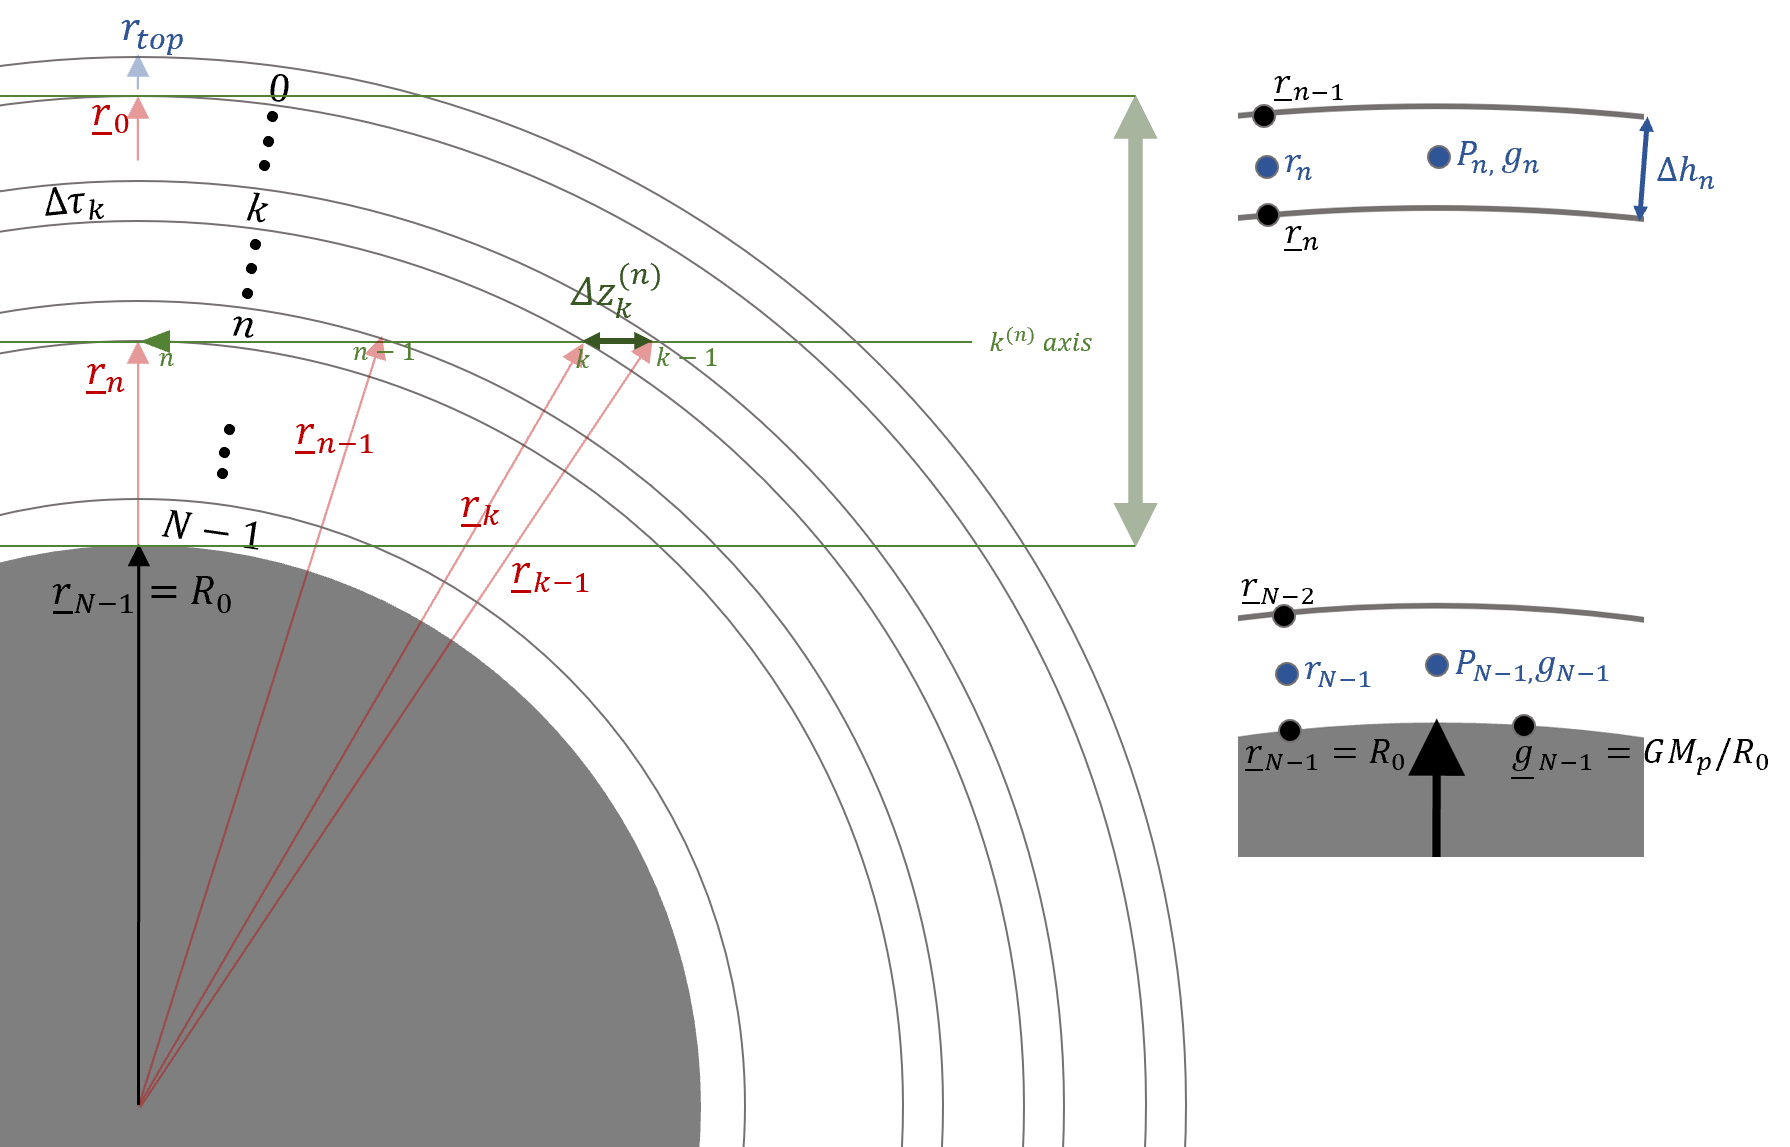
\includegraphics[width=1.0\linewidth]{fig/transmission_coord.PNG}
\caption{レイヤーモデルにおける光学的厚さの計算方向。\label{fig:transmission_coord}}
\end{center}
\end{figure*}
